\chapter{常见的曲面}
\section{曲面及其方程}
\subsection{曲面的方程的定义}
\noindent
\thispagestyle{empty}
\begin{enumerate}[]
	\setlength{\itemindent}{1em}
	\setlength{\topsep}{0.01em}
	\setlength{\itemsep}{0.01em}
	\item 从几何上看,曲面可以看作是具有{\color{dy}某种约束的点的几何轨迹};
	\item 从解析上看,约束条件通常用一个{\color{dy}三元二次方程$S:F(x,y,z)=0$}表示.
\end{enumerate}
\defination[曲面的方程]\index{QMDFC@曲面的方程}
曲面$S$表示为点的集合:
\begin{equation}
S=\left\lbrace (x,y,z)\in \mathbb{R}^3|F(x,y,z)=0\right\rbrace 
\end{equation}
\par 其特点为:
\begin{enumerate}[(1)]
	\setlength{\itemindent}{3em}
	\setlength{\topsep}{0.01em}
	\setlength{\itemsep}{0.01em}
	\item 曲面上的点都满足方程;
	\item 满足方程的点都在曲面上,不满足方程的点都不在曲面上.
\end{enumerate}
\subsection{曲面方程举例}
\begin{enumerate}[1.]
	\setlength{\topsep}{0.01em}
	\setlength{\itemsep}{0.01em}
	\item {\color{dy}平面\index{PM@平面}}
	\begin{enumerate}[(1)]
		\setlength{\topsep}{0.01em}
		\setlength{\itemsep}{0.01em}
		\item 约束条件:动点到定点的连线始终与一定直线垂直。
		\item 一般方程:$Ax+By+Cz+D=0.$
	\end{enumerate}
	\item {\color{dy}球面\index{QM@球面}}\label{球面}
	\begin{enumerate}[(1)]
		\setlength{\topsep}{0.01em}
		\setlength{\itemsep}{0.01em}
		\item 约束条件:动点($M(x,y,z)$)到定点(球心$M_0(x_0,y_0,z_0)$)的距离始终为常数(半径$R$)。
		\item 一般方程:$(x-x_0)^2+(y-y_0)^2+(z-z_0)^2=R^2.$
	\end{enumerate}
	\newpage
	\item {\color{dy}圆柱面\index{YZM@圆柱面}}\label{圆柱面}
	\begin{enumerate}[(1)]
		\setlength{\topsep}{0.01em}
		\setlength{\itemsep}{0.01em}
		\item 约束条件:到一定直线的距离等于常数($R$)的动点的轨迹方程。
		\item 定直线为$z$轴的方程:$x^2+y^2=R^2.$
	\end{enumerate}
	\item {\color{dy}圆锥面\index{YZM@圆锥面}}\label{圆锥面}
	\begin{enumerate}[(1)]
		\setlength{\topsep}{0.01em}
		\setlength{\itemsep}{0.01em}
		\item 约束条件:动点与一定直线上某定点的连线始终与该定直线交成等角$\varphi $。
		\item 定直线$z$轴,其上的定点为原点的方程:$z^2=\cot^2 \varphi(x^2+y^2).$
	\end{enumerate}
\end{enumerate}
\subsection{曲面的两个基本问题}
\begin{enumerate}[1.]
	\setlength{\itemindent}{2em}
	\setlength{\topsep}{0.01em}
	\setlength{\itemsep}{0.01em}
	\item 已知曲面作为点的几何轨迹时,求曲面方程;
	\item 已知一个三元方程$F(x,y,z)=0,$研究它所表示的几何形状.
\end{enumerate}

\subsection{构建曲面方程的一般步骤}
\begin{enumerate}[1.]
	\setlength{\itemindent}{2em}
	\setlength{\topsep}{0.01em}
	\setlength{\itemsep}{0.01em}
	\item 针对实际问题,{\color{dy}建立合适的空间直角坐标系};
	\item 先在曲面上任取一{\color{dy}动点$M(x,y,z)$},再依据题意,{\color{dy}找到约束条件,建立等量关系},(即利用数学解析语言描述几何约束条件)得到{\color{dy}关于动点$M$的坐标变量$x,y,z$的等式};
	\item 整理得到{\color{dy}曲面的方程}.
\end{enumerate}

\subsection{柱坐标与球坐标}
\label{柱坐标}
\noindent
\tdefination[柱坐标]\index{ZZB@柱坐标}
空间直角坐标系中点$M(x,y,z).$
\begin{enumerate}[(1)]
	\setlength{\itemindent}{3em}
	\setlength{\topsep}{0.01em}
	\setlength{\itemsep}{0.01em}
	\item 它在$xOy$面上的投影点$N(x,y,0)$;
	\item 用极坐标系表示点$N(\rho ,\theta ,0)$.
\end{enumerate}
\par 那么我们称三元有序数组$(\rho ,\theta ,z)$为点$M$的{\color{dy}柱坐标}.如图\ref{柱坐标1}.
\begin{enumerate}[]
	\setlength{\topsep}{0.01em}
	\setlength{\itemsep}{0.01em}
	\item {\color{dy}柱坐标与直角坐标的关系}
	\begin{equation}
	\begin{cases}
	x=\rho \cos\theta,\\
	y=\rho \sin\theta ,\\
	z=z.
	\end{cases}
	\quad 
	\begin{array}{l}
	0 \le \rho < +\infty\\
	0 \le \theta \le 2\pi \quad \mbox{或} \quad  -\pi \le \theta \le \pi\\
	-\infty < z < +\infty\\
	\end{array}
	\end{equation}
							{\color{dy}柱坐标系\index{ZZBX@柱坐标系}}是极坐标系添加$z$轴坐标得到的空间坐标系.
				\item {\color{dy}柱坐标的坐标曲面}
	\begin{enumerate}[]
		\setlength{\itemindent}{1em}
		\setlength{\topsep}{0.01em}
		\setlength{\itemsep}{0.01em}
		\item $\rho = \rho_0 $:以$z$轴为中心轴,半径为$\rho_0$的{\color{dy}圆柱面};
		\item $\theta =\theta_0$:从$z$轴出发且从$x$轴的转角为$\theta_0$的{\color{dy}半平面};
		\item $z =z_0$:过$z$轴上点$z_0$且与$z$轴垂直的{\color{dy}平面};
	\end{enumerate}
	点$M(\rho_0,\theta_0,z_0)$是这三个曲面的交点.
\end{enumerate}


	\begin{figure}[h]
\begin{center}
	\subfigure[柱坐标]{
	\begin{minipage}[b]{0.4\linewidth}
		\centering
		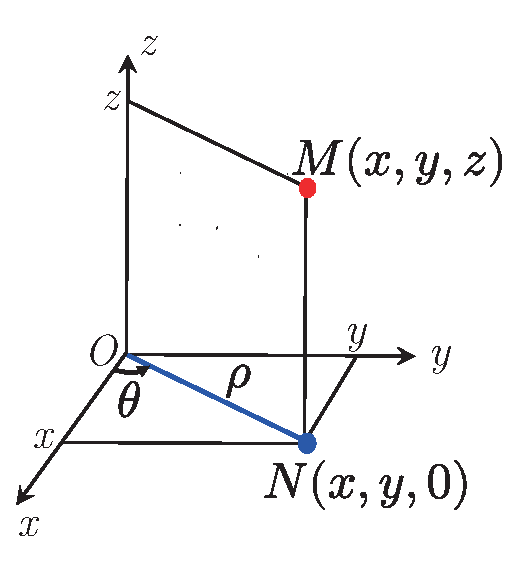
\includegraphics[width=0.85\linewidth]{picture/C-3/柱坐标1.eps}
		\label{柱坐标1}
	\end{minipage}
}
\subfigure[球坐标]{
	\begin{minipage}[b]{0.4\linewidth}
		\centering
		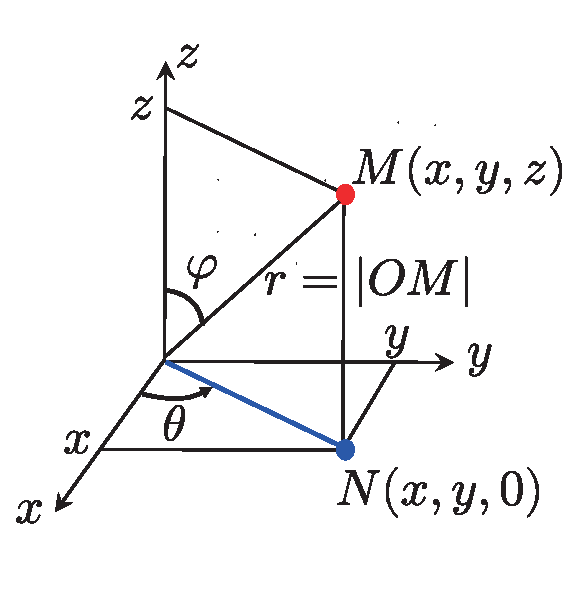
\includegraphics[width=0.9\linewidth]{picture/C-3/球坐标1.eps}
		\label{球坐标1}
	\end{minipage}
}
\caption{球坐标与柱坐标}
\end{center}
\end{figure}

\defination[球坐标]\index{QZB@球坐标}
空间直角坐标系中点$M(x,y,z).$
\begin{enumerate}[(1)]
	\setlength{\itemindent}{3em}
	\setlength{\topsep}{0.01em}
	\setlength{\itemsep}{0.01em}
	\item 它在$xOy$面上的投影点$N(x,y,0)$;
	\item 用$r$表示点$M$到原点$O$的距离;
	\item 用$\varphi $表示$\overrightarrow{OM}$到$z$轴正向的夹角;
	\item 用$\theta $表示从$x$轴正向到原点$\overrightarrow{ON}$的转角.
\end{enumerate}
\par 那么我们称三元有序数组$(r ,\varphi ,\theta )$为点$M$的{\color{dy}球坐标}.如图\ref{球坐标1}.
\begin{enumerate}[]
	\setlength{\topsep}{0.01em}
	\setlength{\itemsep}{0.01em}
	\item {\color{dy}球坐标与直角坐标的关系}
	\begin{equation}
	\begin{cases}
	x=r\sin \varphi  \cos\theta,\\
	y=r\sin \varphi  \sin\theta ,\\
	z=r\cos \varphi.
	\end{cases}
	\quad 
	\begin{array}{l}
	0 \le r < +\infty\\ 
	0 \le \theta \le 2\pi \quad \mbox{或} \quad -\pi \le \theta \le \pi \\ 
	0 \le \varphi \le \pi\\ 
	\end{array} 
	\end{equation}
	\item {\color{dy}球坐标的坐标曲面}
	\begin{enumerate}[]
		\setlength{\itemindent}{1em}
		\setlength{\topsep}{0.01em}
		\setlength{\itemsep}{0.01em}
		\item $r = r_0 $:以原点为球心,半径为$r_0$的{\color{dy}球面};
		\item $\varphi  =\varphi_0$:顶点在原点$O$,半顶角为$\varphi_0$的{\color{dy}圆锥面};
		\item $\theta =\theta_0$:从$z$轴出发且从$x$轴的转角为$\theta_0$的{\color{dy}半平面};
	\end{enumerate}
	点$M(r_0 ,\varphi_0 ,\theta_0 )$是这三个曲面的交点.
\end{enumerate}

\subsection{曲面的参数方程}
\tdefination[曲面的参数方程]\index{QMDCSFC@曲面的参数方程}
一般地,曲面可以用两个参数的方程表示:
\begin{equation}
\begin{cases}
x=x(u,v),\\
y=y(u,v),\\
z=z(u,v)
\end{cases}
\end{equation}
\par 给定参数$(u,v)$的一组值,就能确定曲面上一个点的位置.
\par 曲面就是这些点的集合:
\begin{equation*}
S=\left\lbrace  \left( x(u,v),y(u,v),z(u,v)\right)|u \in \mathbb{R},v \in \mathbb{R} \right\rbrace \quad \huo \quad  S=\left\lbrace  \left(x(u,v),y(u,v),z(u,v) \right) | (u,v) \in D \right\rbrace 
\end{equation*}
\par 其中,$D$是$\mathbb{R}^2$的一个区域,它是参数$(u,v)$的取值范围.以下给出几个例子:

\example[圆柱面的参数方程]
求圆柱面$x^2+y^2=a^2$的参数方程.\\
解:代入\hyperref[柱坐标]{\color{超链接}柱坐标变换}$\displaystyle \begin{cases}
x=\rho \cos\theta \\
y=\rho \sin\theta \\
z=z
\end{cases}$\\
得到圆柱面的柱坐标方程为$S:\rho =a.$,即圆柱面的参数方程为:
\begin{equation*}
S:\begin{cases}
x=a\cos\theta, \\
y=a\sin\theta,\\
z=z.
\end{cases}
\begin{array}{l}
0 \le \theta \le 2\pi \quad \mbox{或} \quad  -\pi \le \theta \le \pi\\
-\infty < z < +\infty\\
\end{array}
\end{equation*}

\newpage
\example[球面的参数方程]
求球面$x^2+y^2+z^2=a^2$的参数方程.\\
解:代入\hyperref[球坐标]{\color{超链接}球坐标变换}$\displaystyle 	\begin{cases}
x=r\sin \varphi  \cos\theta,\\
y=r\sin \varphi  \sin\theta ,\\
z=r\cos \varphi.
\end{cases}$\\
得到圆柱面的柱坐标方程为$S:r =a.$,即圆柱面的参数方程为:
\begin{equation*}
S:	\begin{cases}
x=a\sin \varphi  \cos\theta,\\
y=a\sin \varphi  \sin\theta ,\\
z=a\cos \varphi.
\end{cases}
\begin{array}{l}
0 \le \theta \le 2\pi \quad \mbox{或} \quad -\pi \le \theta \le \pi \\ 
0 \le \varphi \le \pi\\ 
\end{array} 
\end{equation*}

\section{空间曲线的方程}
\subsection{空间曲线的参数方程}
\tdefination[空间曲线的参数方程]\index{QXDCSFC@曲线的参数方程}
空间曲线可以看作是质点的运动轨迹。曲线$C$上动点$M(x,y,z)$表示为
\begin{equation}
\begin{cases}
x=x(t),\\
y=y(t),\\
z=z(t).
\end{cases}
\, a \le t \le b.
\label{空间曲线的参数方程}
\end{equation}
\par 那么式\ref{空间曲线的参数方程}就称为空间曲线$C$的参数方程,其中$t$为参数.(空间曲线参数方程中参数可取时间 、转动角度或其它变量.)以下举两个例子:

\example[直线的参数方程]
{\color{dy}几何意义}\quad 直线可以看作是做匀速直线运动的质点的几何轨迹(速度:$\overrightarrow{v}=(m,n,t)$,时间:$t$).
\par{\color{dy} 参数方程}\quad $\displaystyle L:\begin{cases}
x=x_0+mt,\\
y=y_0+nt,\\
z=z_0+pt.
\end{cases}\, -\infty  < t < +\infty $

\newpage
\example[圆柱螺旋线的参数方程]\index{YZRXX@圆柱螺旋线}
{\color{dy}几何意义}\quad 动点$M$在圆柱面$S:x^2+y^2=R^2$上以等角速度$\omega $绕$z$轴旋转,同时又以线速度$v$沿平行于$z$轴的正向均匀地上升.
\par {\color{dy}参数方程}\quad $\displaystyle L:\begin{cases}
x=R\cos \omega t,\\
y=R\sin \omega t,\\
z=vt.
\end{cases}$
令$\displaystyle \theta =\omega t,b=\frac{v}{\omega}$得:
$\displaystyle L:\begin{cases}
x=R\cos \theta ,\\
y=R\sin \theta,\\
z=b\theta .
\end{cases}\, -\infty  < \theta  < +\infty $

\subsection{空间曲线的一般方程}
\tdefination[空间曲线的一般方程]\index{QXDYBFC@曲线的一般方程}
空间曲线可以看作是两曲面的交线。即
\begin{equation}
C:
\begin{cases}
F(x,y,z)=0,\\
G(x,y,z)=0.
\end{cases}
\end{equation}
{\color{dy}空间曲线一般方程的特点}
\begin{enumerate}[1.]
	\setlength{\itemindent}{2em}
	\setlength{\topsep}{0.01em}
	\setlength{\itemsep}{0.01em}
	\item 空间曲线的一般方程不唯一:可以用任意两个过$C$的曲面$S_1,S_2$的方程联立得到的方程组来表示;
	\item 空间曲线$C$位于曲面$S_1,S_2$方程的线性组合确定的曲面$\Sigma $上:
	\begin{equation}
	\Sigma :\lambda F(x,y,z)+\mu G(x,y,z)=0.\quad (\lambda ,\mu \in \mathbb{R},\lambda^2+\mu^2 \ne 0)
	\end{equation}
\end{enumerate}

\example[空间曲线举例]
方程组$\displaystyle 
\begin{cases}
x^2+y^2+z^2-2Rz=0,\\
x^2+y^2+z^2-R^2=0.
\end{cases}$
表示怎样的曲线?
\begin{enumerate}[1.]
	\setlength{\itemindent}{2em}
	\setlength{\topsep}{0.01em}
	\setlength{\itemsep}{0.01em}
	\item {\color{dy}直接分析}
	\begin{enumerate}[]
		\setlength{\itemindent}{2em}
		\setlength{\topsep}{0.01em}
		\setlength{\itemsep}{0.01em}
		\item $x^2+y^2+z^2-2Rz=0$表示圆心为$(0,0,R)$半径为$R$的球面;
		\item $x^2+y^2+z^2-R^2=0$表示圆心为$(0,0,0)$半径为$R$的球面.
	\end{enumerate}
	即该曲线可以表示为两个球面的交线。
	\item {\color{dy}变形方程后分析 
		$\displaystyle 
		\begin{cases}
		x^2+y^2+z^2=R^2,\\
		z=\displaystyle \frac{1}{2}R.
		\end{cases}$}
	\begin{enumerate}[]
		\setlength{\itemindent}{2em}
		\setlength{\topsep}{0.01em}
		\setlength{\itemsep}{0.01em}
		\item $x^2+y^2+z^2=R^2$表示圆心为$(0,0,R)$半径为$R$的球面;
		\item $z=\displaystyle  \frac{1}{2}R$表示平面.
	\end{enumerate}
	即该曲线也可以表示为球面和平面的交线。
	\item {\color{dy}变形方程后分析 
		$\displaystyle 
		\begin{cases}
		x^2+y^2=\displaystyle \frac{3}{4} R^2,\\
		z=\displaystyle \frac{1}{2}R.
		\end{cases}$}
	\begin{enumerate}[]
		\setlength{\itemindent}{2em}
		\setlength{\topsep}{0.01em}
		\setlength{\itemsep}{0.01em}
		\item $x^2+y^2=\displaystyle \frac{3}{4} R^2$表示对称轴为$z$轴的圆柱面;
		\item $z=\displaystyle  \frac{1}{2}R$表示平面.
	\end{enumerate}
	即该曲线还可以表示为圆柱面和平面的交线。
\end{enumerate}

\example[维维安尼(Viviani)曲线]\index{Viviani@Viviani(维维安尼曲线)}
方程组
\begin{equation*}
\begin{cases}
x^2+y^2+z^2=a^2,\\
x^2+y^2=ax.
\end{cases}
\quad (a>0)
\end{equation*}
\par 的图像是球面$x^2+y^2+z^2=a^2$与母线平行于$z$轴的圆柱面$\displaystyle (x-\frac{a}{2})^2+y^2=\frac{a^2}{4}$的交线,称为{\color{dy}维维安尼(Viviani)曲线},也可以用等价的方程组
\begin{equation*}
\begin{cases}
z^2+ax=a^2,\\
x^2+y^2=ax.
\end{cases}
\quad (a>0)
\end{equation*}
\par 来表示,其中$0 \le x \le a$.
\jg
\subsection{空间圆}\index{KJY@空间圆}
\tdefination[空间圆周]
一般地,一个球面
$$
S:(x-x_0)^2+(y-y_0)^2+(z-z_0)^2=R^2
$$
\par 被平面
$$\pi:Ax+By+Cz+D=0$$
\par 截下一个{\color{dy}空间圆周}\index{KJYZ@空间圆周},当且仅当球心$M_0(x_0,y_0,z_0)$到平面$\pi $的距离$d$小于等于球面半径$R$,即
\begin{equation}
d=\frac{|Ax_0+By_0+Cz_0+D|}{\sqrt{A^2+B^2+C^2}} \le R.
\end{equation}

\theorem[空间圆的圆心和半径]
记圆周上任意一点的矢径为:$\overrightarrow{r}=(x,y,z)$圆周的圆心的矢径为:$\overrightarrow{r_0}=(x_0,y_0,z_0)$,则球面的向量式和\hyperref[平面的向量式法式方程]{\color{超链接}平面的向量式法式方程}分别为:
\begin{equation*}
\begin{array}{l}
S:(\overrightarrow{r}-\overrightarrow{r_0})\cdot (\overrightarrow{r}-\overrightarrow{r_0})=R^2\\
\pi : \overrightarrow{n_0} \cdot \overrightarrow{r}-p=0\quad (|\overrightarrow{n_0}=1|)
\end{array}
\end{equation*}

\begin{enumerate}[]
	\setlength{\itemindent}{2em}
	\setlength{\topsep}{0.01em}
	\setlength{\itemsep}{0.01em}
	\item {\color{dy}原理} \quad 空间圆轴$C$的圆心就是过球心且垂直于$\pi$的直线与$\pi $的交点.
	\item {\color{dy}表达式} \jg \quad
	$
	\begin{cases}
	\overrightarrow{r}=\overrightarrow{r_0}+t\overrightarrow{n},\\
	\overrightarrow{n_0} \cdot \overrightarrow{r}-p=0.
	\end{cases}
	\Longleftrightarrow \, \overrightarrow{r_0}+(p-\overrightarrow{n_0}\cdot \overrightarrow{r_0})\overrightarrow{n_0}.
	$\\
	\jg \hspace*{6em}球心到圆心的距离为
	$
	d=|p-\overrightarrow{n} \cdot \overrightarrow{r_0}| \le R.
	$\\
	\jg 综上,{\color{dy}圆心的矢径}为:$\overrightarrow{r_0}+(p-\overrightarrow{n_0}\cdot \overrightarrow{r_0})\overrightarrow{n_0}$.\\
	\jg  {\color{dy}空间圆的半径}为:$r=\sqrt{R^2-d^2}=\sqrt{R^2-(p-\overrightarrow{n} \cdot \overrightarrow{r_0})^2}$
\end{enumerate}

\section{柱面}
\subsection{柱面的定义}
\tdefination[柱面]
在空间中,由平行于定方向且与一条定曲线相交的一族平行直线所构成的曲面叫做{\color{dy}柱面}\index{ZM1@柱面!ZM@柱面}.
\par 从几何上看,柱面就是由一条平行于直线 $L$ 的直线沿曲线 $C$ 连续平移而形成的{\color{dy}平行直线族}.\index{PXZSC@平行直线族}\\
其中,
\sj
\begin{enumerate}[]
	\setlength{\itemindent}{2em}
	\setlength{\topsep}{0.01em}
	\setlength{\itemsep}{0.01em}
	\item 动直线$L$ 叫做柱面的{\color{dy}直母线}\index{ZM1@柱面!ZMX@直母线},
	\item 定曲线$C$叫做柱面的{\color{dy}准线}\index{ZM1@柱面!ZX@准线},
	\item 平行于动直线的方向$\overrightarrow{v}$叫做{\color{dy}直母线方向}\index{ZM1@柱面!ZMXFX@直母线方向}.
\end{enumerate}
注意:柱面的准线不是唯一的,与每一条母线都相交的曲线都可以作为柱面的准线.

\subsection{柱面方程}
\ttheorem[柱面的一般方程]\index{ZM1@柱面!ZMDYBFC@柱面的一般方程}

\par {\color{dy}已知}:准线$C:
\begin{cases}
F(x,y,z)=0,\\
G(x,y,z)=0
\end{cases}$
和母线的方向向量$\overrightarrow{v}=(m,n,p)$\\
\par {\color{dy}原理}:在柱面上取动点$M(x,y,z)$,作平行于母线的方向$\overrightarrow{v}$的直线交准线$C$于点$N(u,v,w).$由\hyperref[点向式方程]{\color{超链接}直线的点向式方程}(平行向量的条件)和点在曲面上可以得到。
\par {\color{dy}表达式}:
\begin{equation}
\begin{cases}
\displaystyle \frac{x-u}{m}=\frac{y-v}{n}=\frac{z-w}{p}=t,\\
F(u,v,w)=0.\\
G(u,v,w)=0.\\
\end{cases}
\Longrightarrow \quad 
S:
\begin{cases}
F(x-mt,y-nt,z-pt)=0.\\
G(x-mt,y-nt,z-pt)=0.
\end{cases}
\end{equation}
\par 消去参数$t$可以得到柱面的一般方程。

\theorem[柱面的参数方程]\index{ZM1@柱面!ZMDCSFC@柱面的参数方程}

\par {\color{dy}已知}:准线$C:
\begin{cases}
x=u(t),\\
y=v(t),\\
z=w(t).
\end{cases}$
和母线的方向向量$\overrightarrow{v}=(m,n,p)$\\
\par {\color{dy}原理}:在柱面上取动点$M(x,y,z)$,作平行于母线的方向$\overrightarrow{v}$的直线交准线$C$于点$N(u(t),v(t),w(t)).$由\hyperref[直线的参数方程]{\color{超链接}直线的参数方程}可以得到。
\par {\color{dy}表达式}:
\begin{equation}
S:\begin{cases}
x=u(t)+ms,\\
y=v(t)+ns,\\
z=w(t)+ps.
\end{cases}
\quad (-\infty<t,s<+\infty)
\end{equation}

\example[特殊的柱面方程]

\par  一般地,方程$F(x,y)=0$在$Oxyz$空间表示柱面$S$,在$xOz$平面表示曲线$C$.
\par {\color{dy}方程特点}:方程中不含变量$z$.
\par {\color{dy}几何特点}:柱面$S$上点$M(x,y,z)$在$xOy$面上的投影点$N(x,y,0)$在曲面$C$上.\\
\hspace*{7em}柱面的母线平行于$z$轴.\\
\hspace*{7em}柱面的准线为$xOy$平面上的曲线$C$.
\par 总结如下
\begin{center}
\begin{tabular}{|c|c|c|}
	\hline
	方程 &母线   &  准线    \\
	\hline
	 \hspace*{1em} $F(x,y)=0$ \hspace*{1em} &\hspace*{1em} 平行于$z$轴  \hspace*{1em}  & \hspace*{1em}  在$xOy$平面上的曲线
	$C:
	\begin{cases}
	F(x,y)=0,\\
	z=0
	\end{cases}
	$ \hspace*{1em}  \\
	\hline
\hspace*{1em} $G(y,z)=0$ \hspace*{1em}  &\hspace*{1em} 平行于$x$轴  \hspace*{1em}  & \hspace*{1em}  在$yOz$平面上的曲线
$C:
\begin{cases}
G(y,z)=0,\\
x=0
\end{cases}
$  \hspace*{1em}  \\
	\hline
\hspace*{1em} $H(x,z)=0$ \hspace*{1em} &\hspace*{1em} 平行于$y$轴  \hspace*{1em}  & \hspace*{1em} 在$zOx$平面上的曲线
$C:
\begin{cases}
H(x,z)=0,\\
y=0
\end{cases}
$\hspace*{1em} \\
	\hline
\end{tabular}
\end{center}

\section{锥面} 
\subsection{锥面的定义}
\tdefination[锥面]\index{ZM2@锥面!ZM2@锥面}
\par 在空间中,由曲线$C$上的点与不在 $C$ 上的一个定点 $M_0$ 的连线组成的曲面称为{\color{dy}锥面} .
\par 从几何上看,锥面就是由过同一定点 $M_0$的动直线 $L$沿曲线 $C$连续滑动而形成的{\color{dy}相交直线族}.\\
其中,
\sj
\begin{enumerate}[]
	\setlength{\itemindent}{2em}
	\setlength{\topsep}{0.01em}
	\setlength{\itemsep}{0.01em}
	\item 定点$M_0$ 叫做锥面的{\color{dy}顶点}\index{ZM2@锥面!DD@顶点},
	\item 动直线$L$ 叫做锥面的{\color{dy}直母线}\index{ZM2@锥面!ZMX@直母线},
	\item 定曲线$C$叫做锥面的{\color{dy}准线}\index{ZM2@锥面!ZX@准线}.
\end{enumerate}
注意:锥面的准线不是唯一的,与每一条母线都相交的曲线都可以作为锥面的准线.

\subsection{一般锥面的方程}

\ttheorem[锥面的一般方程]\index{ZM2@锥面!ZMDYBFC@锥面的一般方程}

\par {\color{dy}已知}:锥面的顶点$M_0(x_0,y_0,z_0)$,准线$C:
\begin{cases}
F(x,y,z)=0,\\
G(x,y,z)=0.
\end{cases}$
\par {\color{dy}原理}:连接点$M_0,M$的直线交曲线$C$于点$N(u,v,w)$,由\hyperref[两点式方程]{\color{超链接}直线的两点式方程}在及点在曲线上可以得到,即
\begin{equation*}
\begin{cases}
\displaystyle \frac{u-x_0}{x-x_0}=\frac{v-y_0}{y-y_0}=\frac{w-z_0}{z-z_0}=t,\\
F(u,v,w)=0,\\
G(u,v,w)=0.
\end{cases}
\end{equation*}
\par {\color{dy}表达式}:
\begin{equation}
	S:
	\begin{cases}
	F(x_0+(x-x_0)t,y_0+(y-y_0)t,z_0+(z-z_0)t)=0,\\
	G(x_0+(x-x_0)t,y_0+(y-y_0)t,z_0+(z-z_0)t)=0.
	\end{cases}
\end{equation}

\theorem[锥面的参数方程]\index{ZM2@锥面!ZMDCSFC@锥面的参数方程}

\par {\color{dy}已知}:锥面的顶点$M_0(x_0,y_0,z_0)$,准线$C:
\begin{cases}
x=u(t),\\
y=v(t),\\
z=w(t).
\end{cases}$
\par {\color{dy}原理}:连接点$M_0,M$的直线交曲线$C$于点$N(u(t),v(t),w(t))$,由\hyperref[两点式方程]{\color{超链接}直线的两点式方程}和\hyperref[直线的参数方程]{\color{超链接}直线的参数方程}及点在曲线上可以得到,即
\begin{equation*}
\displaystyle \frac{u(t)-x_0}{x-x_0}=\frac{v(t)-y_0}{y-y_0}=\frac{w(t)-z_0}{z-z_0}=t.\\
\end{equation*}
\par {\color{dy}表达式}:
\begin{equation}
S:
\begin{cases}
x=x_0+(u(t)-x_0)s,\\
y=y_0+(v(t)-y_0)s,\\
z=z_0+(w(t)-z_0)s.
\end{cases}
\quad (-\infty <t,s<+\infty )
\end{equation}

\example[特殊的锥面方程]
\begin{table}[h]
\begin{center}
\begin{tabular}{|c|c|}
	\hline
	名称 &方程 \\
	\hline
	  \hspace*{1em} $S:z^2=(x^2+y^2)$ \hspace*{1em} & 圆锥面(夹角为$90^{\circ}$)  \\
	\hline
\hspace*{1em} $S:xy+yz+zx=0$ \hspace*{1em}   & 圆锥面 \\
	\hline
\multirow{2}{*}{\hspace*{1em} $\displaystyle S:\frac{x^2}{a^2}+\frac{y^2}{b^2}-\frac{z^2}{c^2}=0$ \hspace*{1em}}  &\multirow{2}{*}{椭圆锥面(渐进锥面)}   \\
	& \\
	\hline
\end{tabular}
	\caption{特殊的锥面方程}
	\label{特殊的锥面方程}
\end{center}
\end{table}
\sj
\subsection{锥面方程的特点}
\tdefination[齐次方程]
如果对于任意非零实数$t$,函数$F(x,y,z)$满足
\begin{equation}
F(tx,ty,tz)=t^nF(x,y,z)
\end{equation}
其中,$n$为整数.则称函数$F(x,y,z)$为关于$x,y,z$的{\color{dy}$\, \,  n$次齐次函数}.\index{QCHS@齐次函数}
\par 方程$F(x,y,z)=0$为关于$x,y,z$的{\color{dy}$\, \,  n$次齐次方程}.\index{QCFC@齐次方程}
	\par 观察表\ref{特殊的锥面方程}可以发现方程中每一项都是二次的,称为二次齐次方程.令$F(x,y,z=xy+yz+zx)$,则有二次齐次函数:
	$$
	F(tx,ty,tz)=t^2F(x,y,z)
	$$
	
	\theorem[原点为顶点的锥面方程的特点]
	以坐标原点为顶点的锥面方程$\Longleftrightarrow$ $x, y, z$的齐次方程 .\\
原理:利用$F(tx,ty,tz)=t^nF(x,y,z)=0 \Longleftrightarrow  F(tx,ty,tz)=F(x,y,z)=0$
\\$ \Longleftrightarrow$若点$M$在曲面上,则由原点$O$和点$M$所确定的直线也在曲面上.\colorbox{文字底色}{(解析语言$\Longleftrightarrow$几何语言)}

	\addinference[一般锥面方程的特点]
以点$M_0(x_0,y_0,z_0)$为顶点的锥面方程$\Longleftrightarrow$ $(x-x_0), (y-y_0), (z-z_0)$的齐次方程 .\\

\section{旋转曲面}\label{旋转曲面}
\subsection{旋转曲面的定义}
\tdefination[旋转曲面]
一条空间曲线$C$绕一条定直线$L$旋转一周所得到的曲面$S$称为{\color{dy}旋转曲面}\index{XZQM@旋转曲面}.
\\其中,
\begin{enumerate}[]
	\setlength{\itemindent}{2em}
	\setlength{\topsep}{0.01em}
	\setlength{\itemsep}{0.01em}
	\item 定直线$L$称为旋转曲面的{\color{dy}旋转轴}.\index{XZQM@旋转曲面!XZZ@旋转轴}
	\item 曲线$C$称为旋转曲面的{\color{dy}母线}.\index{XZQM@旋转曲面!MX@母线}
	\item 母线$C$上每个点$M_0$绕旋转轴 $L$旋转得到一个圆,称为{\color{dy}纬圆}.\index{XZQM@旋转曲面!WY@纬圆}(纬圆与轴垂直)
	\item 过旋转轴$L$的半平面与旋转面$S$ 的交线称为{\color{dy}经线}\index{XZQM@旋转曲面!JX@经线}({\color{dy}子午线}\index{XZQM@旋转曲面!ZWX@子午线}).(经线可以作为母线,但母线未必是经线.)
\end{enumerate}

\subsection{旋转曲面的方程}
\ttheorem[特殊情况的旋转曲面方程]
母线为$yOz$面上的曲线 $C:f(y,z)= 0$ ,旋转轴为$z$轴 .在旋转曲面$S$上取动点$M(x,y,z)$,过点$M$作纬圆交母线$C$于点$N(x_0,y_0,z_0)$.则
\begin{equation*}
S:
\begin{cases}
x_0=0\\
z_0=z\\
\sqrt{x^2+y^2}=|y_0|
\end{cases}
\Longrightarrow
\begin{cases}
y_0=\pm \sqrt{x^2+y^2}\\
z_0=z
\end{cases}
\end{equation*}
将上式代入$f(y_0,z_0)$得:$S:f(\pm \sqrt{x^2+y^2},z)=0$,类似地,我们可以得到
\begin{table}[h]
	\begin{center}
		\begin{tabular}{|c|c|c|}
			\hline
			母线&旋转轴  &旋转曲面方程  \\
			\hline
			\multirow{2}{*}{\hspace*{1cm}$yOz$面上的曲线$C:f(y,z)=0$} \hspace*{1cm}& $z$轴 & \hspace*{1cm}$S:f(\pm  \sqrt{x^2+y^2},z)=0$  \hspace*{1cm}\\
			\cline{2-3}
			&$y$轴   & \hspace*{1cm}$S:f(y,\pm  \sqrt{x^2+z^2})=0$ \hspace*{1cm}\\
			\hline
			\multirow{2}{*}{\hspace*{1cm}$xOz$面上的曲线$C:f(x,z)=0$\hspace*{1cm}} & $z$轴 &  \hspace*{1cm} $S:f(\pm  \sqrt{x^2+y^2},z)=0$ \hspace*{1cm}\\
			\cline{2-3}
			& $x$轴 &\hspace*{1cm} $S:f(x,\pm  \sqrt{y^2+z^2})=0$  \hspace*{1cm} \\
			\hline
			\multirow{2}{*}{\hspace*{1cm}$xOy$面上的曲线$C:f(x,y)=0$\hspace*{1cm}} & $y$轴 &  \hspace*{1cm} $S:f(\pm  \sqrt{x^2+z^2},y)=0$ \hspace*{1cm}\\
			\cline{2-3}
			& $x$轴 & \hspace*{1cm} $S:f(x,\pm  \sqrt{y^2+z^2})=0$  \hspace*{1cm} \\
			\hline
		\end{tabular}
\end{center}
\caption{母线在坐标平面内、旋转轴为坐标轴的旋转曲面方程}
\label{特殊情况的旋转曲面方程}
\end{table}

\ttheorem[旋转曲面的一般方程]\index{XZQM@旋转曲面!XZQMDYBFC@旋转曲面的一般方程}
\par {\color{dy}已知}:在旋转曲面$S$上取动点$M(x,y,z)$,过点$M$作垂直于旋转轴$L=(m,n,t)$的平面$\pi $,交轴$L$于点$Q$,交母线$
C:
\begin{cases}
	F(x,y,z)=0\\
	G(x,y,z)=0
\end{cases}
$于点$N(u,v,w)$,取轴上一定点$M_0(x_0,y_0,z_0)$.\\
(即需知道{\color{dl}1. 旋转轴上一点};{\color{dl}2. 旋转轴的方向向量};{\color{dl}3. 母线方程})
\par {\color{dy}原理}:旋转曲面的定义
\begin{equation*}
\begin{cases}
\mbox{点}N\mbox{在母线上}\\
\mbox{平面与轴垂直}\\
\mbox{轴上一点到垂直与轴的纬圆上任意一点的距离始终相等}
\end{cases}
\,\, \Longleftrightarrow \, \,
\begin{cases}
N \in C \\
\overrightarrow{NM}  \, \bot \,  \overrightarrow{v}\\
|M_0M|=|M_0N|
\end{cases}
\end{equation*}
\par {\color{dy}表达式}:
\begin{equation}
S:
	\begin{cases}
	F(u,v,w)=0,\\
	G(u,v,w)=0,\\
	m(x-u)+n(y-v)+t(z-w)=0,\\
	(x-x_0)^2+(y-y_0)^2+(z-z_0)^2=(u-x_0)^2+(v-y_0)^2+(z-z_0)^2
	\end{cases}
\end{equation}
消去参数$u,v,w$即可得到旋转曲面的一般方程.

\newpage

\theorem[旋转曲面的参数方程]\index{XZQM@旋转曲面!XZQMDCSFC@旋转曲面的参数方程}
空间曲线
$$\Gamma:
\begin{cases}
x=x(t),\\
y=y(t),\\
z=z(t)\\
\end{cases}
\quad 
\alpha \le t \le \beta
$$
绕$z$轴选择所得到的旋转曲面$S$的方程.
\par {\color{dy}已知}:在旋转曲面$S$上取动点$M(x,y,z)$,过点$M$作纬圆$C$位于平面$\pi :z=z(t)$上,设其圆心为点$Q$,半径为$r(t)$
\par {\color{dy}原理}:$r(t)=\sqrt{x^2(t)+y^2(t)}.$,类似于\hyperref[柱坐标]{\color{超链接}柱坐标变换},先定$t$求出每一个$t$对应的纬圆方程,再让$t$在定义的范围内摆动(即一个个连续的纬圆形成一个曲面).
\par {\color{dy}表达式}:
\begin{equation}
S:
\begin{cases}
x=\sqrt{x^2(t)+y^2(t)}\, \cos \theta,\\
y=\sqrt{x^2(t)+y^2(t)}\, \sin \theta,\\
z=z(t)
\end{cases}
\quad 
\theta \in [0,2\pi],\,
\alpha \le t \le \beta
\end{equation}

\section{常见的二次曲面}
\subsection{二次曲面的定义}
\tdefination[二次曲面]\index{ECQM@二次曲面}
三元二次方程
\begin{equation}
a_1 x^2 + a_2 y^2 + a_3 z^2 +b_1 xy +b_2 yz+b_3 zx + c_1x+c_2y+c_3z+d=0
\end{equation}
所确定的曲面称为{\color{dy}二次曲面},其中二次项系数不全为$0$.

\jg
\subsection{二次曲面的基本类型}

\begin{enumerate}
	\setlength{\itemindent}{0em}
	\setlength{\topsep}{0.01em}
	\setlength{\itemsep}{0.01em}
	\item  \link[旋转曲面]:\link[球面]、\link[旋转椭球面]、\link[圆柱面]、\link[圆锥面]、\link[旋转椭球面]、\link[旋转单叶双曲面]、\link[旋转双叶双曲面]、\link[旋转抛物面].(注:圆环面不是二次曲面)
	\item  \link[椭球面]、\link[双曲面]、\link[抛物面]、\link[二次锥面]和\link[二次柱面].
\end{enumerate}

\newpage
\subsection{二次曲面的性质}
对称性
\begin{table}[!h]
	\begin{minipage}[!h]{\columnwidth}
		\centering
		\begin{tabular}{|c|c|}
				\hline
			\kg 方程条件\kg & \kg  曲面对称性 \kg\\
			\hline
			\kg $F(x,y,z)=F(x,y,-z)$\kg & \kg 关于$xOy$面对称\kg \\
			\hline
			\kg $F(x,y,z)=F(-x,y,z)$ \kg & \kg 关于$yOz$面对称\kg \\
			\hline
			\kg $F(x,y,z)=F(x,-y,z)$ \kg & \kg 关于$zOx$面对称\kg \\
			\hline
		\end{tabular}
	\caption{二次曲面关于面的对称性}
	\label{二次曲面关于面的对称性}
	\end{minipage}
	\\[12pt]%设置两个表格之间的空白行距离
	\begin{minipage}[h]{\columnwidth}
		\centering
		\begin{tabular}{|c|c|}
			\hline
			\kg 方程条件 \kg &  \kg  曲面对称性 \kg\\
			\hline
			\kg $F(x,y,z)=F(x,-y,-z)$ \kg & \kg 关于$x$轴对称 \kg \\
			\hline
			\kg $F(x,y,z)=F(-x,y,-z)$\kg & \kg 关于$y$轴对称 \kg  \\
			\hline
			\kg $F(x,y,z)=F(-x,-y,z)$ \kg & \kg 关于$z$轴对称 \kg \\
			\hline
		\end{tabular}
	\caption{二次曲面关于轴的对称性}
	\label{二次曲面关于轴的对称性}
	\end{minipage}
	\\[12pt]%设置两个表格之间的空白行距离
\begin{minipage}[h]{\columnwidth}
	\centering
	\begin{tabular}{|c|c|}
		\hline
		\kg 方程条件 \kg & \kg  曲面对称性 \kg \\
		\hline
		\kg $F(x,y,z)=F(-x,-y,-z)$ \kg & \kg 关于原点对称 \kg \\
		\hline
	\end{tabular}
	\caption{二次曲面关于原点的对称性}
	\label{二次曲面关于原点的对称性}
\end{minipage}
	\vspace{-0.1cm}%设置第二个表格与正文下文的空白行距离
\end{table}

\subsection{椭球面}\index{TQM@椭球面}\label{椭球面}
\sja
\begin{enumerate}
	\setlength{\itemindent}{0em}
	\setlength{\topsep}{0.01em}
	\setlength{\itemsep}{0.01em}
	\item 椭球面的基本定义与基本方程
\jg

\enbelowdefination[椭球面]
\hspace*{1em} 方程$\displaystyle S:\frac{x^2}{a^2}+\frac{y^2}{b^2}+\frac{z^2}{c^2}=1$所表示的曲面称为中心在原点的{\color{dy}椭球面}.该方程称为{\color{dy}椭球面的标准方程}\index{TQM@椭球面!TQMDBZFC@椭球面的标准方程}.其中$a,b,c$为正的常数,称为椭球面的{\color{dy}半轴}\index{TQM@椭球面!BZ@半轴}.
\par {\color{dy}特殊情况}
\sja
\begin{enumerate}
	\setlength{\itemindent}{1em}
	\setlength{\topsep}{0.01em}
	\setlength{\itemsep}{0.01em}
	\item 当$a=b=c$时,表示球面:$S:x^2+y^2+z^2=a^2$.
	\item 当$a=b$时表示{\color{dy}旋转椭球面}\index{TQM@椭球面!XZTQM@旋转椭球面}\label{旋转椭球面}:$ \displaystyle S:\frac{x^2+y^2}{a^2}+\frac{z^2}{c^2}=1$.
\end{enumerate}

\enbelowtheorem[椭球面的一般方程]
\hspace*{1em} 方程
\begin{equation}
\Sigma : \frac{(x-x_0)^2}{a^2}+\frac{(y-y_0)^2}{b^2}+\frac{(z-z_0)^2}{c^2}=1
\end{equation}
所表示的曲面称为中心在点$(x_o,y_0,z_0)$的{\color{dy}椭球面}.该方程称为{\color{dy}椭球面的一般方程}\index{TQM@椭球面!TQMDBZFC@椭球面的一般方程}其中$a,b,c$为正的常数,称为椭球面的{\color{dy}半轴}.

\item 椭球面$\displaystyle S:\frac{x^2}{a^2}+\frac{y^2}{b^2}+\frac{z^2}{c^2}=1$的几何性质
\begin{enumerate}
	\setlength{\topsep}{0.01em}
	\setlength{\itemsep}{0.01em}
	\item 对称性\\
	\kg \kg 由表$\,$\ref{二次曲面关于面的对称性}  $-$ \ref{二次曲面关于原点的对称性}$\,$可知椭球面关于各坐标面、坐标轴及原点都对称 .
	
	\item 有界性\\
	\kg \kg 椭球面上的点$(x,y,z)$满足:
	\begin{equation*}
	\begin{cases}
	\displaystyle  \frac{x^2}{a^2}\le 1,\\
	\displaystyle  \frac{y^2}{b^2} \le 1,\\
	\displaystyle  \frac{z^2}{c^2} \le 1. 
	\end{cases}
\quad \Longleftrightarrow \quad
	\begin{cases}
	|x| \le a,\\
	|y| \le b,\\
	|z| \le c.
	\end{cases}
	\end{equation*}
	$\Longleftrightarrow$椭圆包含在由六个平面$x=\pm a,y=\pm b,z=\pm c$所围成的长方体.
\end{enumerate}

\item  椭球面$\displaystyle S:\frac{x^2}{a^2}+\frac{y^2}{b^2}+\frac{z^2}{c^2}=1$的平截线
\jg

\enbelowdefination[平截线]
\kg 平行于坐标面的平面截曲面的截痕线称作{\color{dy}平截线}\index{PJX@平截线}.
\begin{enumerate}
	\setlength{\itemindent}{1em}
	\setlength{\topsep}{0.01em}
	\setlength{\itemsep}{0.01em}
	\item 截平面:与$xOy$平行的平面$ z = h $ \\ 
	\kg 平截线方程:
	\begin{equation*}
	\begin{cases}
	\displaystyle \frac{x^2}{a^2} + \frac{y^2}{b^2}=1- \frac{h^2}{c^2}\\
	x=h \, (|h|<c)
	\end{cases}
	\quad \Longrightarrow \quad 
	\begin{cases}
	\displaystyle \frac{x^2}{\frac{a^2(c^2-h^2)}{c^2}} + \frac{y^2}{\frac{b^2(c^2-h^2)}{c^2}}=1\\
	x=h \, (|h|<c)
	\end{cases}
	\end{equation*}
	 \kg 平截线图形:中心点在$z$轴,半轴分别为$\displaystyle \frac{a}{c}\sqrt{c^2-h^2},\frac{b}{c}\sqrt{c^2-h^2}$的椭圆
	
	\item 截平面:与$yOz$平行的平面$ x = m $\\
	\kg 平截线方程:
	\begin{equation*}
	\begin{cases}
	\displaystyle \frac{y^2}{b^2} + \frac{z^2}{c^2}=1- \frac{m^2}{a^2}\\
	x=m\,(|m|<a)
	\end{cases}
	\quad \Longrightarrow \quad 
	\begin{cases}
	\displaystyle \frac{y^2}{\frac{b^2(a^2-m^2)}{m^2}} + \frac{z^2}{\frac{c^2(a^2-m^2)}{m^2}}=1\\
	x=m \, (|m|<a)
	\end{cases}
	\end{equation*}
	\kg 平截线图形:中心点在$x$轴,半轴分别为$\displaystyle \frac{b}{a}\sqrt{a^2-m^2},\frac{c}{a}\sqrt{a^2-m^2}$的椭圆
	
	\item 截平面:与$zOx$平行的平面$ y = k $\\
	\kg 平截线方程:
	\begin{equation*}
	\begin{cases}
	\displaystyle \frac{x^2}{a^2} + \frac{z^2}{c^2}=1- \frac{k^2}{b^2}\\
	y=k \, (|k|<b)
	\end{cases}
	\quad \Longrightarrow \quad 
		\begin{cases}
	\displaystyle \frac{x^2}{\frac{a^2(b^2-k^2)}{b^2}} + \frac{z^2}{\frac{c^2(b^2-k^2)}{b^2}}=1\\
	y=k \, (|k|<b)
	\end{cases}
	\end{equation*}
	\kg 平截线图形:中心点在$y$轴,半轴分别为$\displaystyle \frac{a}{b}\sqrt{b^2-k^2},\frac{c}{b}\sqrt{b^2-k^2}$的椭圆
\end{enumerate}

\end{enumerate}

\subsection{双曲面}\index{SQM@双曲面}\label{双曲面}
\sja
\begin{enumerate}
	\setlength{\itemindent}{0em}
	\setlength{\topsep}{0.01em}
	\setlength{\itemsep}{0.01em}
	\item 单叶双曲面的基本定义与基本方程
	\vspace*{0.5em}
	
\enbelowdefination[单叶双曲面]\index{SQM@双曲面!DYSQX@单叶双曲面}
\kg 方程$\displaystyle S:\frac{x^2}{a^2}+\frac{y^2}{b^2}-\frac{z^2}{c^2}=1$表示的曲面称为中心在原点的{\color{dy}单叶双曲面}.该方程称为{\color{dy}单叶双曲面的标准方程}\index{SQM@双曲面!DYSQXDBZFC@单叶双曲面的标准方程}.其中$a,b,c$为正的常数,称为单叶双曲面的{\color{dy}半轴}.
\par {\color{dy}特殊情况}
\kg 当$a=b$时表示{\color{dy}旋转单叶双曲面}\label{旋转单叶双曲面}$\displaystyle S:\frac{x^2+y^2}{a^2}-\frac{z^2}{c^2}=1.$

	\item 单叶双曲面的几何性质
	\sja
	\begin{enumerate}
		\setlength{\topsep}{0.01em}
		\setlength{\itemsep}{0.01em}
		
		\item 对称性 
		\kg 由表$\,$\ref{二次曲面关于面的对称性}  $-$ \ref{二次曲面关于原点的对称性}$\,$可知单叶双曲面关于各坐标面、坐标轴及原点都对称.
		
		\item 有界性 \kg  单叶双曲面无界
		
		\item 与三坐标平面的交线
		
		\begin{enumerate}
			\setlength{\topsep}{0.01em}
			\setlength{\itemsep}{0.01em}
			\item 与$xOy$平面的交线为椭圆(称为腰椭圆\index{SQM@双曲面!YTY@腰椭圆}):
			\begin{equation}
			C_{xOy}:
			\begin{cases}
			\displaystyle \frac{x^2}{a^2}+\frac{y^2}{b^2}=1,\\
			z=0
			\end{cases}
			\label{S1.1}
			\end{equation}
			
			\item 与$yOz$平面的交线为双曲线(实轴为$y$轴,虚轴为$z$轴):
			\begin{equation}
			C_{yOz}:
			\begin{cases}
			\displaystyle \frac{y^2}{b^2}-\frac{z^2}{c^2}=1,\\
			x=0
			\end{cases}
			\label{S1.2}
			\end{equation}
			
			\item 与$zOx$平面的交线为双曲线(实轴为$x$轴,虚轴为$z$轴):
			\begin{equation}
			C_{zOx}:
			\begin{cases}
			\displaystyle \frac{x^2}{a^2}-\frac{z^2}{c^2}=1,\\
			y=0
			\end{cases}
			\label{S1.3}
			\end{equation}
		\end{enumerate}
		
		\item 平截线
		\begin{enumerate}
			\setlength{\topsep}{0.01em}
			\setlength{\itemsep}{0.01em}
			\item 与平行于$ xOy $面的平面$z = h$的交线是一族椭圆:
			\begin{equation}
			C_{xOy}(h):
			\begin{cases}
			\displaystyle \frac{x^2}{a^2}+\frac{y^2}{b^2}=1+\frac{h^2}{c^2},\\
			z=h
			\end{cases}
			\end{equation}
			其顶点$\displaystyle (\pm a \, \sqrt{1+\frac{h^2}{c^2}},0,h)$和$\displaystyle (0,\pm b \, \sqrt{1+\frac{h^2}{c^2}},h)$分别在双曲线\eqref{S1.2}和双曲线\eqref{S1.3}上.
			\newpage
			\item 与平行于$zOx$面的平面$ y = k $的交线:
			\begin{equation}
			C_{zOx}(k):
			\begin{cases}
			\displaystyle \frac{x^2}{a^2}-\frac{z^2}{c^2}=1-\frac{k^2}{b^2},\\
			y=k
			\end{cases}
			\end{equation}
			\par 当$|k|>b$时,平截线是实轴平行于$z$轴的双曲线,虚轴平行于$x$轴的双曲线.
			\par 当$|k|<b$时,平截线是实轴平行于$x$轴的双曲线,虚轴平行于$z$轴的双曲线.
			\par 当$|k|=b$时,平截线是两条直线:
			$
			\begin{cases}
			\displaystyle \frac{x}{a} \pm \frac{z}{c}=0\\
			y=b
			\end{cases}
			\huo \quad
			\begin{cases}
			\displaystyle \frac{x}{a} \pm \frac{z}{c}=0\\
			y=-b
			\end{cases}
			$
			\item 与平行于$yOz$面的平面$ x = m $的情形与ii类似.
		\end{enumerate}
\end{enumerate}
	
		\item 双叶双曲面的基本定义与基本方程
	\vspace*{0.5em}
	
	\enbelowdefination[双叶双曲面]\index{SQM@双曲面!SYSQX@双叶双曲面}
	\kg 方程$\displaystyle S:\frac{x^2}{a^2}+\frac{y^2}{b^2}-\frac{z^2}{c^2}=-1$表示的曲面称为中心在原点的{\color{dy}双叶双曲面}.该方程称为{\color{dy}单叶双曲面的标准方程}\index{SQM@双曲面!SYSQXDBZFC@双叶双曲面的标准方程}.其中$a,b,c$为正的常数,称为双叶双曲面的{\color{dy}半轴}.
	\par {\color{dy}特殊情况}
	\kg 当$a=b$时表示{\color{dy}旋转双叶双曲面}\label{旋转双叶双曲面}$\displaystyle S:\frac{x^2+y^2}{a^2}-\frac{z^2}{c^2}=-1.$
	
	\item 双叶双曲面的几何性质
	\sja
	\begin{enumerate}
		\setlength{\topsep}{0.01em}
		\setlength{\itemsep}{0.01em}
		
		\item 对称性 
		\kg 由表$\,$\ref{二次曲面关于面的对称性}  $-$ \ref{二次曲面关于原点的对称性}$\,$可知双叶双曲面关于各坐标面、坐标轴及原点都对称.
		
		\item 有界性 \kg  双叶双曲面无界
		
		\item 与三坐标平面的交线
		
		\begin{enumerate}
	\setlength{\topsep}{0.01em}
	\setlength{\itemsep}{0.01em}
	\item 与$xOy$平面的交线为虚椭圆(无交点):
	\begin{equation}
	C_{xOy}:
	\begin{cases}
	\displaystyle \frac{x^2}{a^2}+\frac{y^2}{b^2}=-1,\\
	z=0
	\end{cases}
	\label{S2.1}
	\end{equation}
	
	\item 与$yOz$平面的交线为双曲线(实轴为$z$轴,虚轴为$y$轴):
	\begin{equation}
	C_{yOz}:
	\begin{cases}
	\displaystyle \frac{y^2}{b^2}-\frac{z^2}{c^2}=-1,\\
	x=0
	\end{cases}
	\label{S2.2}
	\end{equation}
	
	\item 与$zOx$平面的交线为双曲线(实轴为$z$轴,虚轴为$x$轴):
	\begin{equation}
	C_{zOx}:
	\begin{cases}
	\displaystyle \frac{x^2}{a^2}-\frac{z^2}{c^2}=-1,\\
	y=0
	\end{cases}
	\label{S2.3}
	\end{equation}
\end{enumerate}

	\newpage

	\item 平截线
		\begin{enumerate}
		\setlength{\topsep}{0.01em}
		\setlength{\itemsep}{0.01em}
		\item 与平行于$ xOy $面的平面$z = h$的交线是一族椭圆:
		\begin{equation}
		C_{xOy}(h):
		\begin{cases}
		\displaystyle \frac{x^2}{a^2}+\frac{y^2}{b^2}=1+\frac{h^2}{c^2},\\
		z=h
		\end{cases}
		\end{equation}
		其顶点$\displaystyle (\pm a \, \sqrt{1+\frac{h^2}{c^2}},0,h)$和$\displaystyle (0,\pm b \, \sqrt{1+\frac{h^2}{c^2}},h)$分别在双曲线\eqref{S1.2}和双曲线\eqref{S1.3}上.

		\item 与平行于$zOx$面的平面$ y = k $的交线:
		\begin{equation}
		C_{zOx}(k):
		\begin{cases}
		\displaystyle \frac{x^2}{a^2}-\frac{z^2}{c^2}=1-\frac{k^2}{b^2},\\
		y=k
		\end{cases}
		\end{equation}
		\par 当$|k|>b$时,平截线是实轴平行于$z$轴的双曲线,虚轴平行于$x$轴的双曲线.
		\par 当$|k|<b$时,平截线是实轴平行于$x$轴的双曲线,虚轴平行于$z$轴的双曲线.
		\par 当$|k|=b$时,平截线是两条直线:
		$
		\begin{cases}
		\displaystyle \frac{x}{a} \pm \frac{z}{c}=0\\
		y=b
		\end{cases}
		\huo \quad
		\begin{cases}
		\displaystyle \frac{x}{a} \pm \frac{z}{c}=0\\
		y=-b
		\end{cases}
		$
		\item 与平行于$yOz$面的平面$ x = m $的情形与ii类似.
	\end{enumerate}
\end{enumerate}
	
\end{enumerate}

\subsection{抛物面}\index{PWM@抛物面}\label{抛物线}
\sja
\begin{enumerate}
	\item 椭圆抛物面的基本定义与基本方程
	
	\enbelowdefination[椭圆抛物面]\index{PWM@抛物面!TYPWM@椭圆抛物面}
	\kg 方程$\displaystyle S:\frac{x^2}{a^2}+\frac{y^2}{b^2}=2z$表示的曲面称为{\color{dy}椭圆抛物面}.该方程称为{\color{dy}椭圆抛物面的标准方程}\index{PWM@抛物面!TYPWMDBZFC@椭圆抛物面的标准方程}.其中$a,b$为正的常数.
	\par {\color{dy}特殊情况}
	\kg 当$a=b$时表示{\color{dy}旋转抛物面}\label{旋转抛物面}$S: x^2+y^2=2a^2z.$
	
	\item 椭圆抛物面的几何性质
		\begin{enumerate}
		\setlength{\topsep}{0.01em}
		\setlength{\itemsep}{0.01em}
		
		\item 对称性 \kg 由表$\,$\ref{二次曲面关于面的对称性}  $-$ \ref{二次曲面关于原点的对称性}$\,$可知椭圆抛物面关于面$xOz,yOz$对称.
		
		\item 有界性 \kg 椭圆抛物面无界.
		
		\item 平截线
			\begin{enumerate}
			\setlength{\topsep}{0.01em}
			\setlength{\itemsep}{0.01em}
			\item 与平行于$xOy$平面的平面$z=h(h>0)$的交线为椭圆:
			\begin{equation*}
			C_{xOy}=
			\begin{cases}
			\displaystyle \frac{x^2}{2ha^2}+\frac{y^2}{2hb^2}=1\\
			z=h
			\end{cases}
			\end{equation*}
			\end{enumerate}
		\end{enumerate}

\item 双曲抛物面的基本定义和基本方程

\enbelowdefination[双曲抛物面]\index{PWM@抛物面!SQPWM@双曲抛物面}
	\kg 方程$\displaystyle S:-\frac{x^2}{a^2}+\frac{y^2}{b^2}=2z$表示的曲面称为{\color{dy}双曲抛物面}(或称为{\color{dy}马鞍面}\index{PWM@抛物面!MAM@马鞍面}).该方程称为{\color{dy}双曲抛物面的标准方程}\index{PWM@抛物面!SQPWMDBZFC@双曲抛物面的标准方程}.其中$a,b$为正的常数.

\item 双曲抛物面的几何性质
		\begin{enumerate}
	\setlength{\topsep}{0.01em}
	\setlength{\itemsep}{0.01em}
	
	\item 对称性 \kg 由表$\,$\ref{二次曲面关于面的对称性}  $-$ \ref{二次曲面关于原点的对称性}$\,$可知双曲抛物面关于面$xOz,yOz$对称.
	
	\item 有界性 \kg 双曲抛物面无界.
	
		\item 与三坐标平面的交线

\begin{enumerate}
	\setlength{\topsep}{0.01em}
	\setlength{\itemsep}{0.01em}
	\item 与$xOy$平面的交线为两条相交直线:
	\begin{equation}
	C_{xOy}:
	\begin{cases}
	\displaystyle \frac{x}{a}+\frac{y}{b}=1,\\
	z=0
	\end{cases}
	\quad
	\begin{cases}
	\frac{x}{a}-\frac{y}{b}=0,\\
	z=0
	\end{cases}
	\end{equation}
	
	\item 与$yOz$平面的交线为开口朝上的抛物线:(顶点:原点$O$,对称轴:$z$轴)
	\begin{equation}
	C_{yOz}:
	\begin{cases}
	y^2=2b^2z,\\
	x=0
	\end{cases}
	\label{P.2}
	\end{equation}
	
	\item 与$zOx$平面的交线为开口朝下的抛物线:(顶点:原点$O$,对称轴:$z$轴)
	\begin{equation}
	C_{zOx}:
	\begin{cases}
	x^2=-2a^2z,\\
	y=0
	\end{cases}
	\label{P.3}
	\end{equation}
\end{enumerate}

\item 平截线
		\begin{enumerate}
			\setlength{\topsep}{0.01em}
			\setlength{\itemsep}{0.01em}
			\item 与平行于$ xOy $面的平面$z = h$的交线:
			\begin{equation}
			C_{xOy}(h):
			\begin{cases}
			\displaystyle -\frac{x^2}{a^2}=2h\\
			z=h.
			\end{cases}
			\end{equation}
			\kg 当$h>0$时,平截线是实轴平行于$y$轴的双曲线,其顶点$(0,\pm b\sqrt{2h},h)$在抛物线\eqref{P.2}上.\\
			\kg 当$h<0$时,平截线是实轴平行于$x$轴的双曲线,其顶点$(\pm a\sqrt{-2h},0,h)$在抛物线\eqref{P.3}上.
			
			\item 与平行于$zOx$面的平面$ y = k $的交线:
			\begin{equation}
			C_{zOx}(k):
			\begin{cases}
			\displaystyle x^2=-2a^2\left(z-\frac{k^2}{2b^2}\right)\\
			y=k.
			\end{cases}
			\end{equation}
			它是开口朝下的抛物线,其顶点$\displaystyle \left(0,k,\frac{k^2}{2b^2}\right)$在抛物线\eqref{P.2}上.

			\item 与平行于$yOz$面的平面$ x = m $的交线:
			\begin{equation}
			C_{yOz}(m):
			\begin{cases}
			\displaystyle y^2=2b^2\left(z+\frac{m^2}{2a^2}\right)\\
			x=m.
			\end{cases}
			\end{equation}
			它是开口朝上的抛物线,其顶点$\displaystyle \left(m,0,-\frac{m^2}{2a^2} \right)$在抛物线\eqref{P.3}上.
		\end{enumerate}
\end{enumerate}
\end{enumerate}

\subsection{二次曲面分类}
	\begin{center}
			\renewcommand\arraystretch{1.5}
		\begin{longtable}{|l|c|c|}% @{\extracolsep{\fill}} 
			%\caption{caption}
			%\label{table:label}  %\\ % add \\ command to tell LaTeX to start a new line
			% Appear table header at the first page as well
			\hline
			\multicolumn{2}{|c|}{曲面类型}         & 标准方程 \\

			\hline
			\endfirsthead
			
			% Appear the table header at the top of every page
			\multicolumn{3}{l}{续表}  \\
			\hline
			\multicolumn{2}{|c|}{曲面类型}         & 标准方程 \\

			\hline
			\endhead
			
			% Appear \hline at the bottom of every page
			\hline
			\endfoot
			
			\multirow{3}{*}{$\,\,$椭球面}   & 椭球面     &   $ S:\displaystyle \frac{x^2}{a^2}+\frac{y^2}{b^2}+\frac{z^2}{c^2}=1. $ \\
			\cline{2-3}
			& 虚椭球面    &  $ S:\displaystyle \frac{x^2}{a^2}+\frac{y^2}{b^2}+\frac{z^2}{c^2}=-1. $   \\
			\cline{2-3}
			& 点       &   $ S:\displaystyle \frac{x^2}{a^2}+\frac{y^2}{b^2}+\frac{z^2}{c^2}=0.(x,y,z=0) $  \\
			\hline
			\multirow{2}{*}{$\,\,$双曲面} & 单叶双曲面   &  $ S:\displaystyle \frac{x^2}{a^2}+\frac{y^2}{b^2}-\frac{z^2}{c^2}=1. $   \\
			\cline{2-3}
			& 双叶双曲面   &   $ S:\displaystyle \frac{x^2}{a^2}+\frac{y^2}{b^2}-\frac{z^2}{c^2}=-1. $ \\
			\hline
			\multicolumn{2}{|c|}{二次锥面}&    \label{二次锥面} \index{ECZM1@二次锥面}         $ S:\displaystyle \frac{x^2}{a^2}+\frac{y^2}{b^2}-\frac{z^2}{c^2}=0. $ \\
			\hline
			\multirow{2}{*}{$\,\,$抛物面}  & 椭圆抛物面   &    $ S:\displaystyle \frac{x^2}{a^2}+\frac{y^2}{b^2}=2z. $\\
			\cline{2-3}
			& 双曲抛物面   &  $ S:\displaystyle \frac{x^2}{a^2}-\frac{y^2}{b^2}=2z. $  \\
			\hline
			\multirow{7}{*}{二次柱面} \label{二次柱面} \index{ECZM2@二次柱面} & 椭圆柱面  \label{椭圆柱面} \index{ECZM2@二次柱面!TYZM@椭圆柱面}  &  $ S:\displaystyle \frac{x^2}{a^2}+\frac{y^2}{b^2}=1. $  \\
			\cline{2-3}
			& 虚椭圆柱面 \label{虚椭圆柱面} \index{ECZM2@二次柱面!XTYZM@虚椭圆柱面}  &   $ S:\displaystyle \frac{x^2}{a^2}+\frac{y^2}{b^2}=-1. $ \\
			\cline{2-3}
			& 直线    &  $ S:\displaystyle \frac{x^2}{a^2}+\frac{y^2}{b^2}=0 $  \\
			\cline{2-3}
			& 双曲柱面  \label{双曲柱面} \index{ECZM2@二次柱面!SQZM@双曲柱面}  &  $ S:\displaystyle \frac{x^2}{a^2}-\frac{y^2}{b^2}=1. $  \\
			\cline{2-3}
			& 一对相交平面  & $ S:\displaystyle \frac{x^2}{a^2}-\frac{y^2}{b^2}=0. $   \\
			\cline{2-3}
			& 抛物柱面 \label{抛物柱面} \index{ECZM2@二次柱面!PWZM@抛物柱面}   &  $ S:\displaystyle x^2=2py $  \\
			\cline{2-3}
			& 一对平行平面  &  $ S:\displaystyle x^2=a^2  (x= \pm a)$   \\
			\multirow{2}{*}{二次柱面} & 一对虚平行平面 &  $ S:\displaystyle x^2=-a^2$  \\
			\cline{2-3}
			& 一对重合平面  &   $ S:\displaystyle x^2=0(x=0)$ \\
		\end{longtable}
	\end{center}
	\renewcommand\arraystretch{1}
	\vspace*{-4em}
\section{直纹面}
\subsection{直纹面的基本定义}\label{直纹面的基本定义}
\tdefination[直纹面]\index{ZWM@直纹面}

如果存在一族直线,使得
\begin{enumerate}[(1)]
	\setlength{\itemindent}{3em}
	\setlength{\topsep}{0.01em}
	\setlength{\itemsep}{0.01em}
	\item 这一族的每一条直线全在$S$上;
	\item $S$上的每一个点都在这一族的某条直线上.
\end{enumerate}
\par 那么称这族直线为曲面$S$的一族{\color{dy}直母线}.在直纹面$S$上任意曲一条与所有直母线相交的曲线$C$,则曲线$C$称为直纹面$S$的{\color{dy}准线}.
\jg
\subsection{直纹面的参数方程}
\ttheorem[直纹面的向量式方程]\index{ZWM@直纹面!ZWMDXLSFC@直纹面的向量式方程}

 {\color{dy}已知}:直纹面$S$的准线$C$的参数方程为
\begin{equation*}
C:\bm{\rho}=\left(\rho_1(u),\rho_2(u),\rho_3(u)\right)
\end{equation*}
\par 设$M(x,y,z)$是直纹面$S$上的动点,过点$M$的直母线$L$交准线$C$与点$N\left(\rho_1(u),\rho_2(u),\rho_3(u)\right)$,设该直母线$L$的方向向量为$\bm{\tau}=\left(\tau_1(u),\tau_2(u),\tau_3(u)\right)$
\par {\color{dy}原理}:连接点$N,M$,则由\link[直纹面的基本定义]以及\link[共线定理2],即$\overrightarrow{NM}=v\,\bm{\tau}$.
\par {\color{dy}表达式}:
\begin{equation}
S:\bm{r}=\overrightarrow{OM}=\overrightarrow{ON}+\overrightarrow{NM}=\bm{\rho}+v \cdot \bm{\tau}.
\label{ZWM.1}
\end{equation}
\par {\color{dy}特殊情况}:
\par \kg \kg 当$\bm{\rho}=\bm{\rho_0}$时,$S$表示锥面;
\par \kg \kg 当$\bm{\tau}=\bm{\tau_0}$时,$S$表示柱面.

\theorem[直纹面的参数方程]\index{ZWM@直纹面!ZWMDCSFC@直纹面的参数方程}
由\link[直纹面的向量式方程]展开得:
\begin{equation}
S:
\begin{cases}
x=\rho_1(u)+v\cdot \tau_1(u),\\
y=\rho_2(u)+v\cdot \tau_2(u),\\
z=\rho_3(u)+v\cdot \tau_3(u).
\end{cases}
\end{equation}
\par {\color{dy}特殊情况}:
锥面
$\begin{cases}
x=x_0+v\cdot \tau_1(u),\\
y=y_0+v\cdot \tau_2(u),\\
z=z_0+v\cdot \tau_3(u).
\end{cases}$
\kg \kg 柱面
$
\begin{cases}
x=\rho_1(u)+m\,v,\\
y=\rho_2(u)+n\,v,\\
z=\rho_3(u)+p\,v.
\end{cases}
$

\subsection{二次非直纹面}
\sj
\begin{table}[h]
		\renewcommand\arraystretch{1.5}
	\begin{center}
		\begin{tabular}{|c|c|c|}
			\hline
			曲面类型 & 曲面方程 & 非直纹面理由\\
			\hline
			\link[椭球面] &$\displaystyle \frac{x^2}{a^2}+\frac{y^2}{b^2}+\frac{z^2}{c^2}=1\,(-1,0)$ & 椭球面是有界的  \\
			\hline 
			\link[双叶双曲面] & $ \displaystyle  \frac{x^2}{a^2}+\frac{y^2}{b^2}-\frac{z^2}{c^2}=1$ & 平行与$xOy$面的直线不全会在曲面上\\
			\hline
			\link[椭圆抛物面] & $\displaystyle  \frac{x^2}{a^2}+\frac{y^2}{b^2}=2z$  &平行与$xOy$面的直线不全会在曲面上\\
			\hline
		\end{tabular}
	\end{center}
	\renewcommand\arraystretch{1}
\end{table}

\subsection{二次直纹面}
\par 二次直纹面有:\link[二次锥面]、\link[二次柱面]、\link[单叶双曲面]、\link[双曲抛物面].

\theorem[单叶双曲面是直纹面]
{\color{dy}原理}:因式分解$+$构建直线族
\begin{equation*}
\begin{aligned}
\displaystyle \frac{x^2}{a^2}+\frac{y^2}{b^2}-\frac{z^2}{c^2}=1
\quad \Longleftrightarrow \quad
\displaystyle \frac{x^2}{a^2}-\frac{z^2}{c^2}=1-\frac{y^2}{b^2}
\quad \Longleftrightarrow \quad
\left(\frac{x}{a}+\frac{z}{c}\right) \left(\frac{x}{a}-\frac{z}{c}\right)= \left(1+\frac{y}{b}\right) \left(1-\frac{y}{b}\right)\\
\Longleftrightarrow \quad
L_{\lambda \mu}:
\begin{cases}
\displaystyle \lambda \left(\frac{x}{a}+\frac{z}{c}\right)=\mu \left(1+\frac{y}{b}\right),\\
\displaystyle \mu \left(\frac{x}{a}-\frac{z}{c}\right)=\lambda \left(1-\frac{y}{b}\right).
\end{cases}
\end{aligned}
\end{equation*}
单叶双曲面有两族直母线:
\begin{equation*}
\begin{cases}
\displaystyle \lambda_1 \left(\frac{x}{a}+\frac{z}{c}\right)=\mu_1 \left(1+\frac{y}{b}\right),\\
\displaystyle \mu_1 \left(\frac{x}{a}-\frac{z}{c}\right)=\lambda_1 \left(1-\frac{y}{b}\right).
\end{cases}
\quad 
\begin{cases}
\displaystyle \lambda_2 \left(\frac{x}{a}+\frac{z}{c}\right)=\mu_2 \left(1-\frac{y}{b}\right),\\
\displaystyle \mu_2 \left(\frac{x}{a}-\frac{z}{c}\right)=\lambda_2 \left(1+\frac{y}{b}\right).
\end{cases}
\end{equation*}

\theorem[双曲抛物面是直纹面]
{\color{dy}原理}:因式分解$+$构建直线族
\begin{equation*}
\displaystyle \frac{x^2}{a^2}-\frac{y^2}{b^2}=2z
\quad \Longleftrightarrow \quad
\left(\frac{x}{a}+\frac{y}{b}\right) \left(\frac{x}{a}-\frac{y}{b}\right)=  2z
\Longleftrightarrow \quad
L_{\lambda \mu}:
\begin{cases}
\displaystyle \lambda \left(\frac{x}{a}+\frac{y}{b}\right)=2 \mu,\\
\displaystyle \mu \left(\frac{x}{a}-\frac{y}{b}\right)=\lambda z.
\end{cases}
\end{equation*}
双曲抛物面有两族直母线:
\begin{equation*}
\begin{cases}
\displaystyle \lambda_1 \left(\frac{x}{a}+\frac{y}{b}\right)=2 \mu_1,\\
\displaystyle \mu_1 \left(\frac{x}{a}-\frac{y}{b}\right)=\lambda_1 z.
\end{cases}
\quad
\begin{cases}
\displaystyle \lambda_2 \left(\frac{x}{a}+\frac{y}{b}\right)=\mu_2 z,\\
\displaystyle \mu_2 \left(\frac{x}{a}-\frac{y}{b}\right)=2 \lambda_2.
\end{cases}
\end{equation*}
\par {\color{dy}两种曲面的直母线都有相同的性质}:

\theorem[直母线性质1]
对单叶双曲面与双曲抛物面,\colorbox{文字底色}{同族的任意两条直母线不共面}.

\theorem[直母线性质2]
对单叶双曲面与双曲抛物面,\colorbox{文字底色}{异族的任意两条直母线共面}.
\\
\par {\color{dy}双曲抛物面的直母线的特殊性质}:

\theorem[双曲抛物面直母线的特殊性质]
双曲抛物面的同族的所有直母线都平行于一个定平面 .\\[9pt]
\kg \kg \kg 
$
\begin{cases}
\displaystyle \lambda_1 \left(\frac{x}{a}+\frac{y}{b}\right)=2 \mu_1,\\
\displaystyle \mu_1 \left(\frac{x}{a}-\frac{y}{b}\right)=\lambda_1 z.
\end{cases}
$
都平行于平面
$\displaystyle \frac{x}{a}+\frac{y}{b}=0.$\\[9pt]
\kg \kg \kg 
$
\begin{cases}
\displaystyle \lambda_2 \left(\frac{x}{a}+\frac{y}{b}\right)=\mu_2 z,\\
\displaystyle \mu_2 \left(\frac{x}{a}-\frac{y}{b}\right)=2 \lambda_2.
\end{cases}
$
都平行于平面
$\displaystyle \frac{x}{a}-\frac{y}{b}=0.$
